\documentclass{llncs}

\usepackage{makeidx} 
\usepackage{makeidx}  % allows for indexgeneration
\usepackage[utf8]{inputenc}
\usepackage{graphicx}
\graphicspath{ {images/} }
\usepackage{url}

\usepackage{balance}       % to better equalize the last page
\usepackage{graphics}      % for EPS, load graphicx instead 
\usepackage[T1]{fontenc}   % for umlauts and other diaeresis
\usepackage{txfonts}
\usepackage[dvipsnames]{xcolor}
\usepackage{booktabs}
\usepackage{textcomp}
\usepackage[flushleft]{threeparttable}
\usepackage{multirow}
\usepackage{placeins}
\usepackage{amssymb}
\usepackage{array}
\usepackage[
backend=biber,
style=ieee,
]{biblatex}
\addbibresource{citation.bib}

\newcommand{\ang}[1]{\textcolor{BrickRed}{[Ang: #1]}}
\newcommand{\keyang}[1]{\textcolor{YellowOrange}{[Keyang: #1]}}
\newcommand{\rosta}[1]{\textcolor{BlueGreen}{[Rosta: #1]}}


\begin{document}

\title{ }
\subtitle{Sentiment Analysis of Facebook Sickle Cell Groups}

\author{Keyang Zheng \and Ang Li \and Rosta Farzan}

\institute{School of Computing and Information \\
    University of Pittsburgh\\
    \email{KEZ20@pitt.edu}}
\maketitle

\begin{abstract}

\end{abstract}

\section{Introduction}

Online health support groups are among the most popular Internet groups, being employed daily to share and seek health-related information, support, and advice. However, it is difficult to discover ways to understand how members in online health support group influence and get influenced by others to adopt a particular medication. While there is an abundance of traces of users' behavior in the online communities, it has been an ongoing challenge to study the impact of online communities on their members beyond the online world since the offline traces are often invisible to researchers. 

In this work, we aim to model impact through sentiment analysis of discussions in online health support groups. The sentiment of online discussions can be a reflection of users' offline state of mind and feelings.  For example, we model the sentiment of discussion, its evolution, and different actors participating in it in online health support groups. Changes in sentiment coupled with other online traces can allows us to connect online-offline interactions. Indeed discussions on the health support groups on Facebook often carry strong sentiment, either positive or negative, which can reflect the real-world challenges and experiences patients and their caregivers face.  We have developed sentiment analysis algorithm to classify the sentiment of each Facebook post and their comments with a high level of accuracy. In this paper, we present our approach in developing such classifier specific to our data.  The classifier allows us to study the group dynamics at the large scale to be able to identify patterns of sentiment changes across the discussion on the group in terms of how it converges or diverges to specific sentiment and what patterns of participation contribute to that.  \rosta{We need to finish this paragraph based on the specific data we will add}

\section{Background}
Include summary of prior research and how it connect to the current paper

\section{Sentiment Analysis}


\subsection{Data Collection}
%In this work, we initially looked at two different support groups on Facebook. One is Sickle Cell Warrior Inc, a public Facebook Page, and the other is Sickle Cell United, a private Facebook Group. According to Facebook itself, a Facebook Page is "designed to be the official profiles for entities, such as celebrities, brands or businesses.", whereas a Facebook Group is "the place for small group communication and for people to share their common interests and express their opinion." Because of this along with the differences in leadership and moderating styles, Sickle Cell Warriors Inc and Sickle Cell United have shown very different group dynamics. And before we started collecting data, both groups' leaders gave us permit to gather the posts and comments for research purposes.

To understand the sentiment of discussions around Sickle Cell Disease (SCD), we analyzed data from a SCD group on Facebook, called Sickle Cell Unite, which started in 2009 by a patient living with sickle cell. It is a closed private Facebook group and each membership request needs to be approved by the group administrators. The messages and content, as shown in Figure \ref{fig:scu}, are only visible to members of the group, and only group members can post or comment.\cite{Farzan2017} \rosta{Add information about Sickle Cell United here with maybe a screenshot}. We used Facebook Graph API to collect data from the Facebook group \footnote{Our data collection is approved by the University of Pittsburgh IRB and is with the permission of the owners of the group}. The data includes all the messages posted for a period of one year, from April 2016 until April 2017. In addition to the original messages, the data includes all the comments in response to each messages and members' liking reactions  to all messages and comments. We also collected the timestamp and the user id associated with each post and comment. The dataset includes 4,862 posts and 26,057 comments associated with those posts. All the posts are in English and some posts contain images or URLs to other web pages. We discarded the images links for the purpose of our sentiment analysis since our algorithm only focuses on text features. Table \ref{tab:descriptive} presents the general descriptives of our dataset

\begin{table}[h!tb]
\centering
\begin{tabular}{lccc}
\toprule
 Total number of posts & 4,862\\
 Total number of comments & 26,057\\
 Number of posts with comments & 3,596\\
 Average number of comments per posts (SD) & 5.38(10.54)\\
 Average length of posts in words (SD) & 43.86(63.35)\\
 Average length of comments in words (SD) & 18.06(30.37)\\
\bottomrule
\end{tabular}
\label{tab:descriptive}
\caption{Descriptive information of the dataset}
\end{table}

\begin{figure}[ht!tb]
\centering
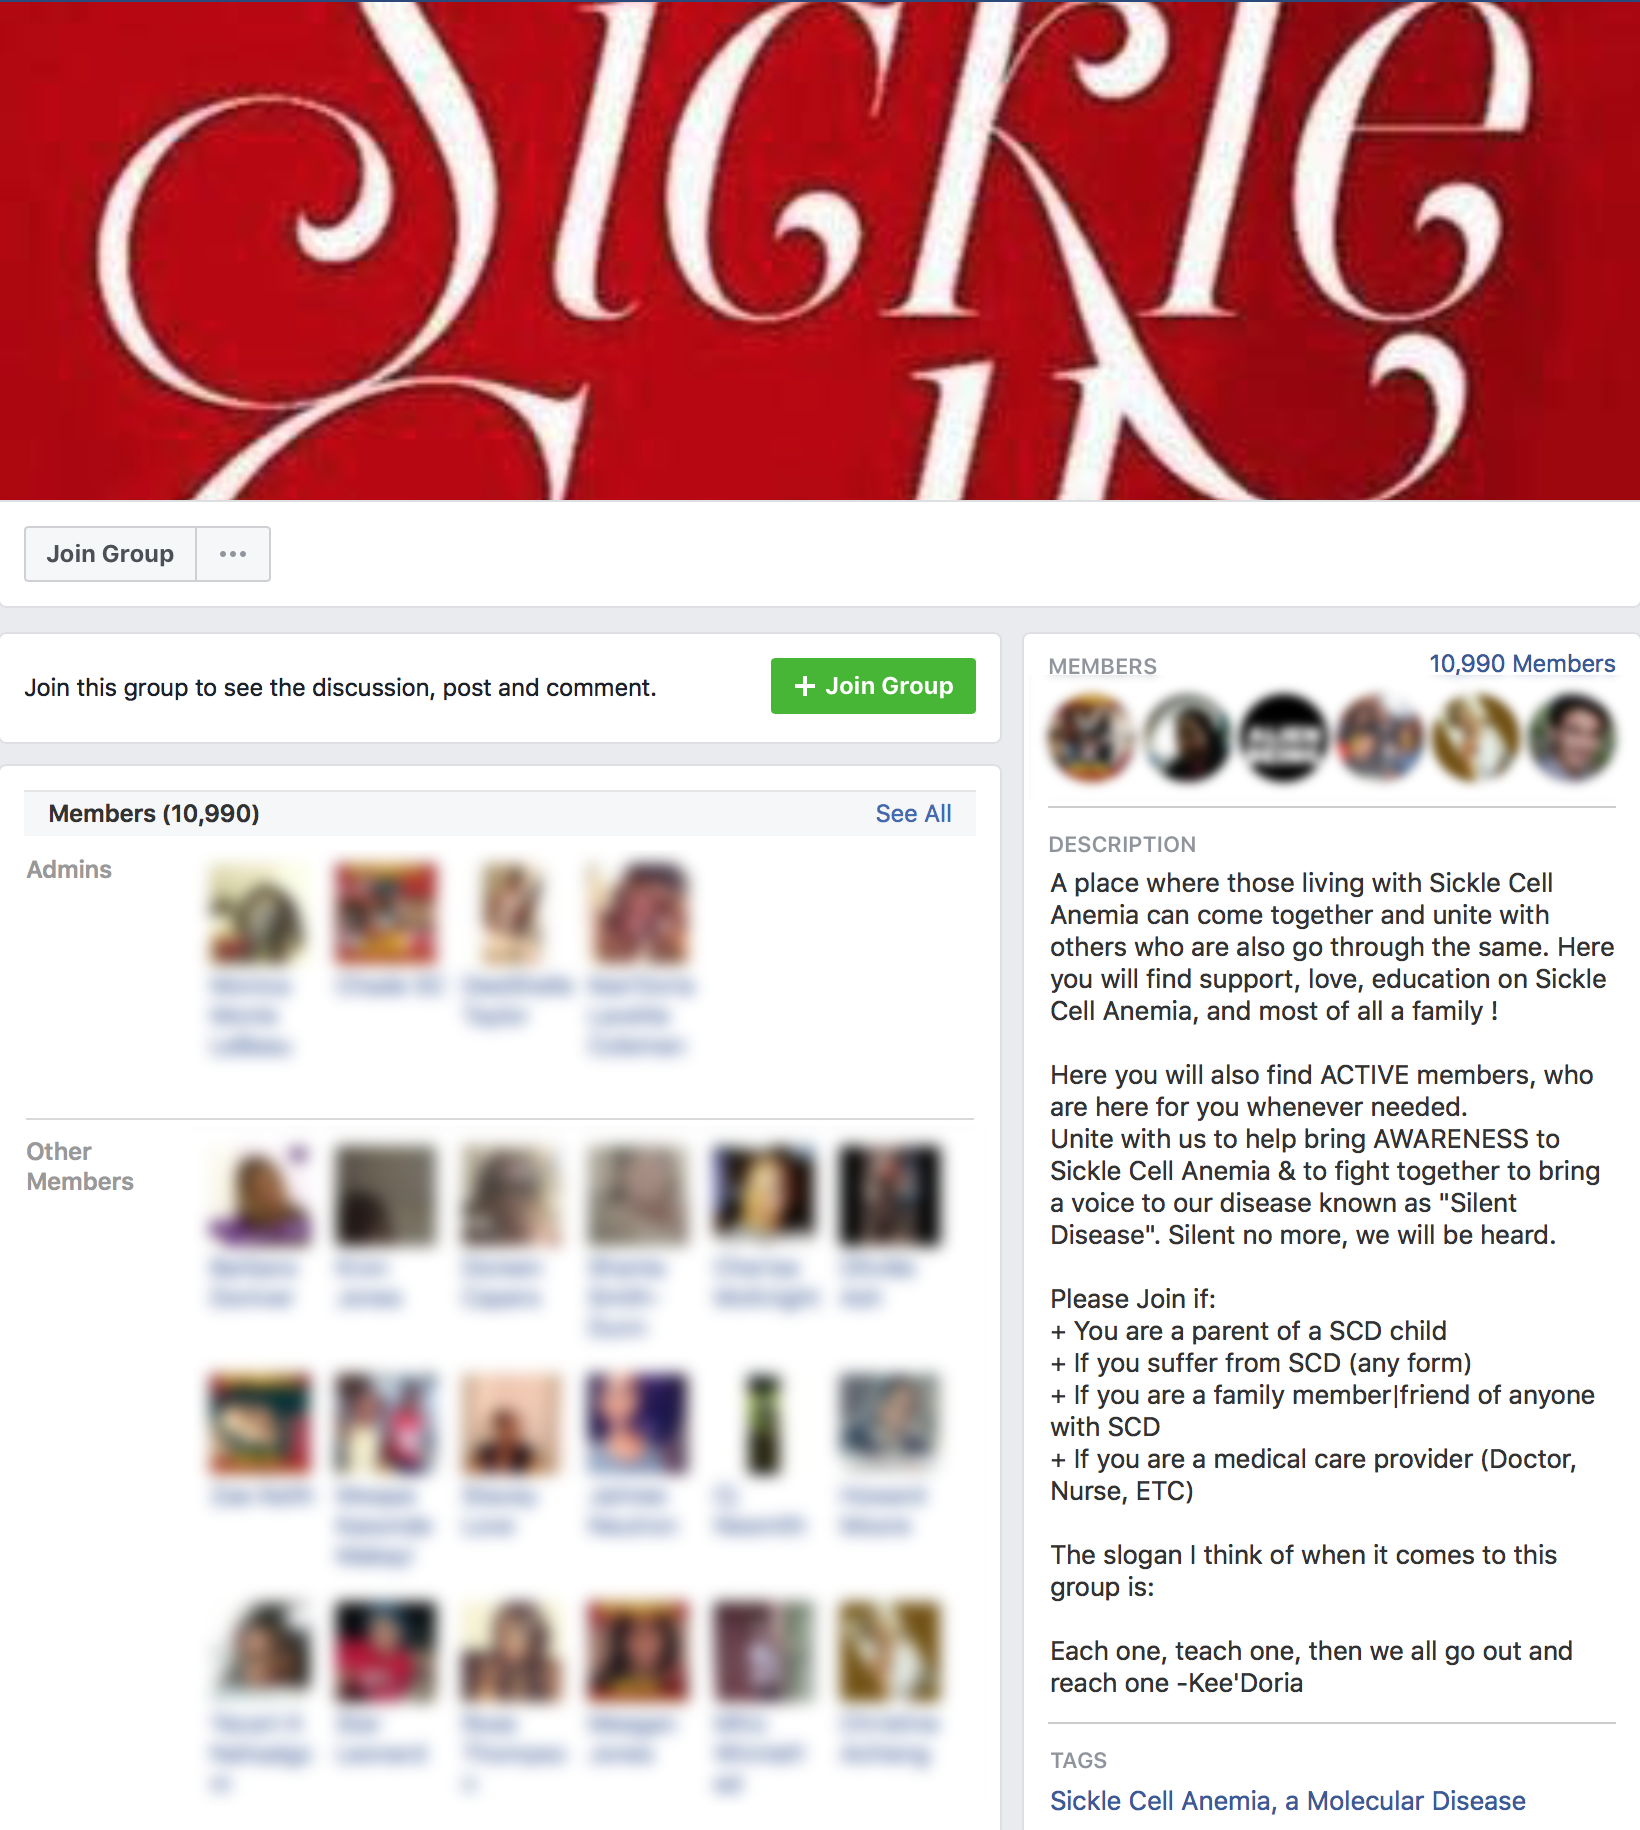
\includegraphics[width=1\textwidth]{scuscreenshot}
\label{fig:scu}
\caption{Screenshot of Sickle Cell Unite}
\end{figure}

%During the cause of analysis, we found that although both groups are considered to be active in term of number of posts and average comments for each post, other factors do affect the results we get. One major factor is the leadership style of both groups' moderators. In previous research, we found that Sickle Cell Warriors Inc is closely moderated by its owner, which caused the data we collected could not reflect the whole picture of how people interact with each other on social media regarding their health issues. Based on these observations, we later decided to focus our analysis on Sickle Cell United. 

\subsection{Supervised Classification Method}

There are a large number of sentiment analysis systems utilizing machine learning methods across different domains such as . However, most approaches are very domain specific and do not well transfer into a new domain \cite{Qiu2011}. In case of SCD Facebook discussions, discussions are often informal and very specific to Sickle Cell, directly using an existing sentiment analysis system is not a desirable choice, yet building a system from the ground up is too time-consuming. We chose to implement a sentiment analysis system based on works from Qiu et al. (2011)\cite{Qiu2011} and Kiritchenko et al. (2014)\cite{Kiritchenko2014}. Both systems use supervised machine learning methods and yield reasonable results. We created our own training data from our data set, extracted features from these messages, and then trained the classification model to fit our unique situation. The fitted model later is applied to all unlabeled messages allowing each to be classified to a sentiment class. 

We also want to get a score indicating the strength of the sentiment each message has. Traditionally, a sentiment score is generated by calculating words' or phrases' semantic orientation from the whole message. This method requires dictionaries of words annotated with its sentiment orientation\cite{Taboada2011}.  However, the result of this approach is independent of the labeling result from our classifier, which contradicts our intention of obtaining a score along side classification result. So we decide to use the probability of the classified class as a proxy for the score. Our classifier is trained to fit each message into positive, negative and neutral three classes, but we want to focus more on just positive and negative classes. So when a message is classified into the neutral class, we pick the higher probability class from positive and negative classes and set the sentiment score of this message to that probability. This method allows us to have the sentiment score covering the whole range from -1 to 1, which helps us later when modeling the sentiment changes and flows. 

As for our training data, it is created after gathering our posts and comments. The training data consists of 494 randomly selected posts and comments from the entire data set. Then we used Mechanical Turk to label each message in our training set into positive, negative or neutral class. Each message was labeled by five independent workers on Mechanical Turk, and later we aggregated the result to determine the class of the message also to reduce the impact of random labeling by a single worker. 



\subsection{Message Features}

All messages were processed before classifier training and applying to the entire data set. Lexical and other semantical features are being extracted during the processing phase. We use two different kinds of lexicon in our system, first is a manually created lexicon (BL lexicon) for positive and negative word lists by Hu \& Liu\cite{Hu2004}, second is an automatically generated word-sentiment association lexicon (Sent140) from Sentiment140 Corpus\cite{go2009twitter} by Kiritchenko, Zhu and Mohammad (2014)\cite{Kiritchenko2014}. The Sent140 lexicon is generated from 1.6 million tweets that being labeled according to emoticons, which provide more coverage of words used in social media compared to more general purposed BL lexicon\cite{Kiritchenko2014}. We also include the mentioning of human body parts, since in the messages involving pains there is a high probability of mentioning certain body parts. In addition, Thelwall et al. (2011) introduced two additional features of PosStrength and NegStrength which convey the strength of emotion displayed in the message\cite{Thelwall2010}. We adopted these features early in our system. The position of a certain word with lexical features is also considered, as intuitively sentiment conveyed at the end of a message has a bigger emphasis compared to the one occurs earlier in the message.\cite{Pang2002} Other semantic features are extracted as well including negation. The lexical features in a negated context are reversed\cite{Taboada2011}, which includes the score from Sent140 lexicon and polarity from BL lexicon. The full lists of features are as follow.
\begin{center}
\begin{tabular}{  m{9em} | m{8cm}  } 
 \hline
 Feature & Definition \\ [0.5ex] 
 \hline\hline
 Name & The number of times a name occurs in the message\\[0.3em]
 Lexicon Score & The sum of score of all the words with a score in Sent140 lexicon in the message\\[0.3em]
 Question Mark & The number of times question marks in the message\\[0.3em]
 Exclamation & The number of times question marks occurs\\[0.3em]
 Post length & The number of words in the message\\[0.3em]
 Average Word Length & The average length of words in the message\\[0.3em]
 Negation & The number of negated context\\[0.3em]
 Last Sentiment & The non-zero score of the last word in a message\\[0.3em]
 Positive Sent140 & The number of words with positive score from Sent140 lexicon contained in the message\\[0.3em]
 Negative Sent140 & The number of words with negative score from Sent140 lexicon contained in the message\\[0.3em]
 Positive BL & The number of positive words from BL lexicon contained in the message\\[0.3em]
 Negative BL & The number of negative words from BL lexicon contained in the message\\[0.3em]
 Human Body Part & Whether a body part is mentioned in the message (1 for yes and 0 of none)\\[0.3em]
 PosStrength & Positive sentiment strength\\[0.3em]
 NegStrength & Negative sentiment strength (The larger of the absolute value the more strength)\\[0.3em]
 \hline
\end{tabular}
\end{center}
Not all the features listed above are used in our final system, as some yield no difference to improve the classification result or being repetitive when using along with other features. 

\subsection{Evaluation and Improvement}
We started to build our classification model with a relatively simple feature set, which included Name, Question Mark, Exclamation, Post Length, Average Word Length, Positive BL, Negative BL, PosStrength, NegStrength. Four different classification models (classifiers) were used: SVM, logistic regression, AdaBoost and Neural Networks\cite{scikit-learn}. However, the result did not yield accurate enough for further analysis. Consider messages were being classified into three classes (positive, negative and neutral), the most accurate result we got was 62\% by using Neural Networks. Confusion Matrix shows all classifiers struggles with neutral messages. Further inspection reveals that misclassifying happens considerably randomly especially with short messages, which occupy a large portion of comments. In order to improve the classification model, we took a closer look at our feature set and decided to adjust the feature set for a better fit of our data set. The Sent140 lexicon is added to address the short and informal language used in social media. Negation is adopted to address the negated context in the message. And the Last Sentiment puts more emphasis on the rare part of the message but also addresses short informal messages in certain levels. PosStrength and NegStrength are dropped because we believe by using Lexicon Score generated by Sent140 lexicon, we already have a viable way to represent the overall strength of the sentiment conveyed by the message. As for Human Body Part, we dropped it in the end despite adding it to address more on negative sentiment,  as we find it actually hurts the accurate.  The same four classification models are used on the new feature set, and the result yields an average 10\% improvement across the board. Close inspection also shows the struggle on short messages has been improved, and misclassification reduced. In the end, we used logistic regression in our model, as it yields the best accuracy in general.

\begin{center}
\begin{tabular}{ m{10em} | m{2cm} | m{2cm} | m{2cm} | m{2cm} }
  \hline
  accuracy & SVM & Logistic Regressio & AdaBoost & Neural Networks\\
  \hline\hline
  Feature Set Original & 0.62 & 0.60 & 0.62 & 0.64\\
  \hline
  Feature Set New & 0.72 & 0.72 & 0.70 & 0.69\\
  \hline
  Feature Set New w/ SentiStrength & 0.70 & 0.73 & 0.70 & 0.71\\
  \hline
  Feature Set New w/ Human Body Parts & 0.71 & 0.71 & 0.71 & 0.68\\
  \hline
\end{tabular}
\end{center}

\section{Results}

\rosta{Can you add the following statistics here:}
Distribution of positive and negative original posts for every month.
\keyang{As shown in the Figure \ref{fig:monthlydistribution}, there is a significant drop of activity when entering 2017, but we do not have any explanations for it.}
\begin{figure}[ht]
\centering
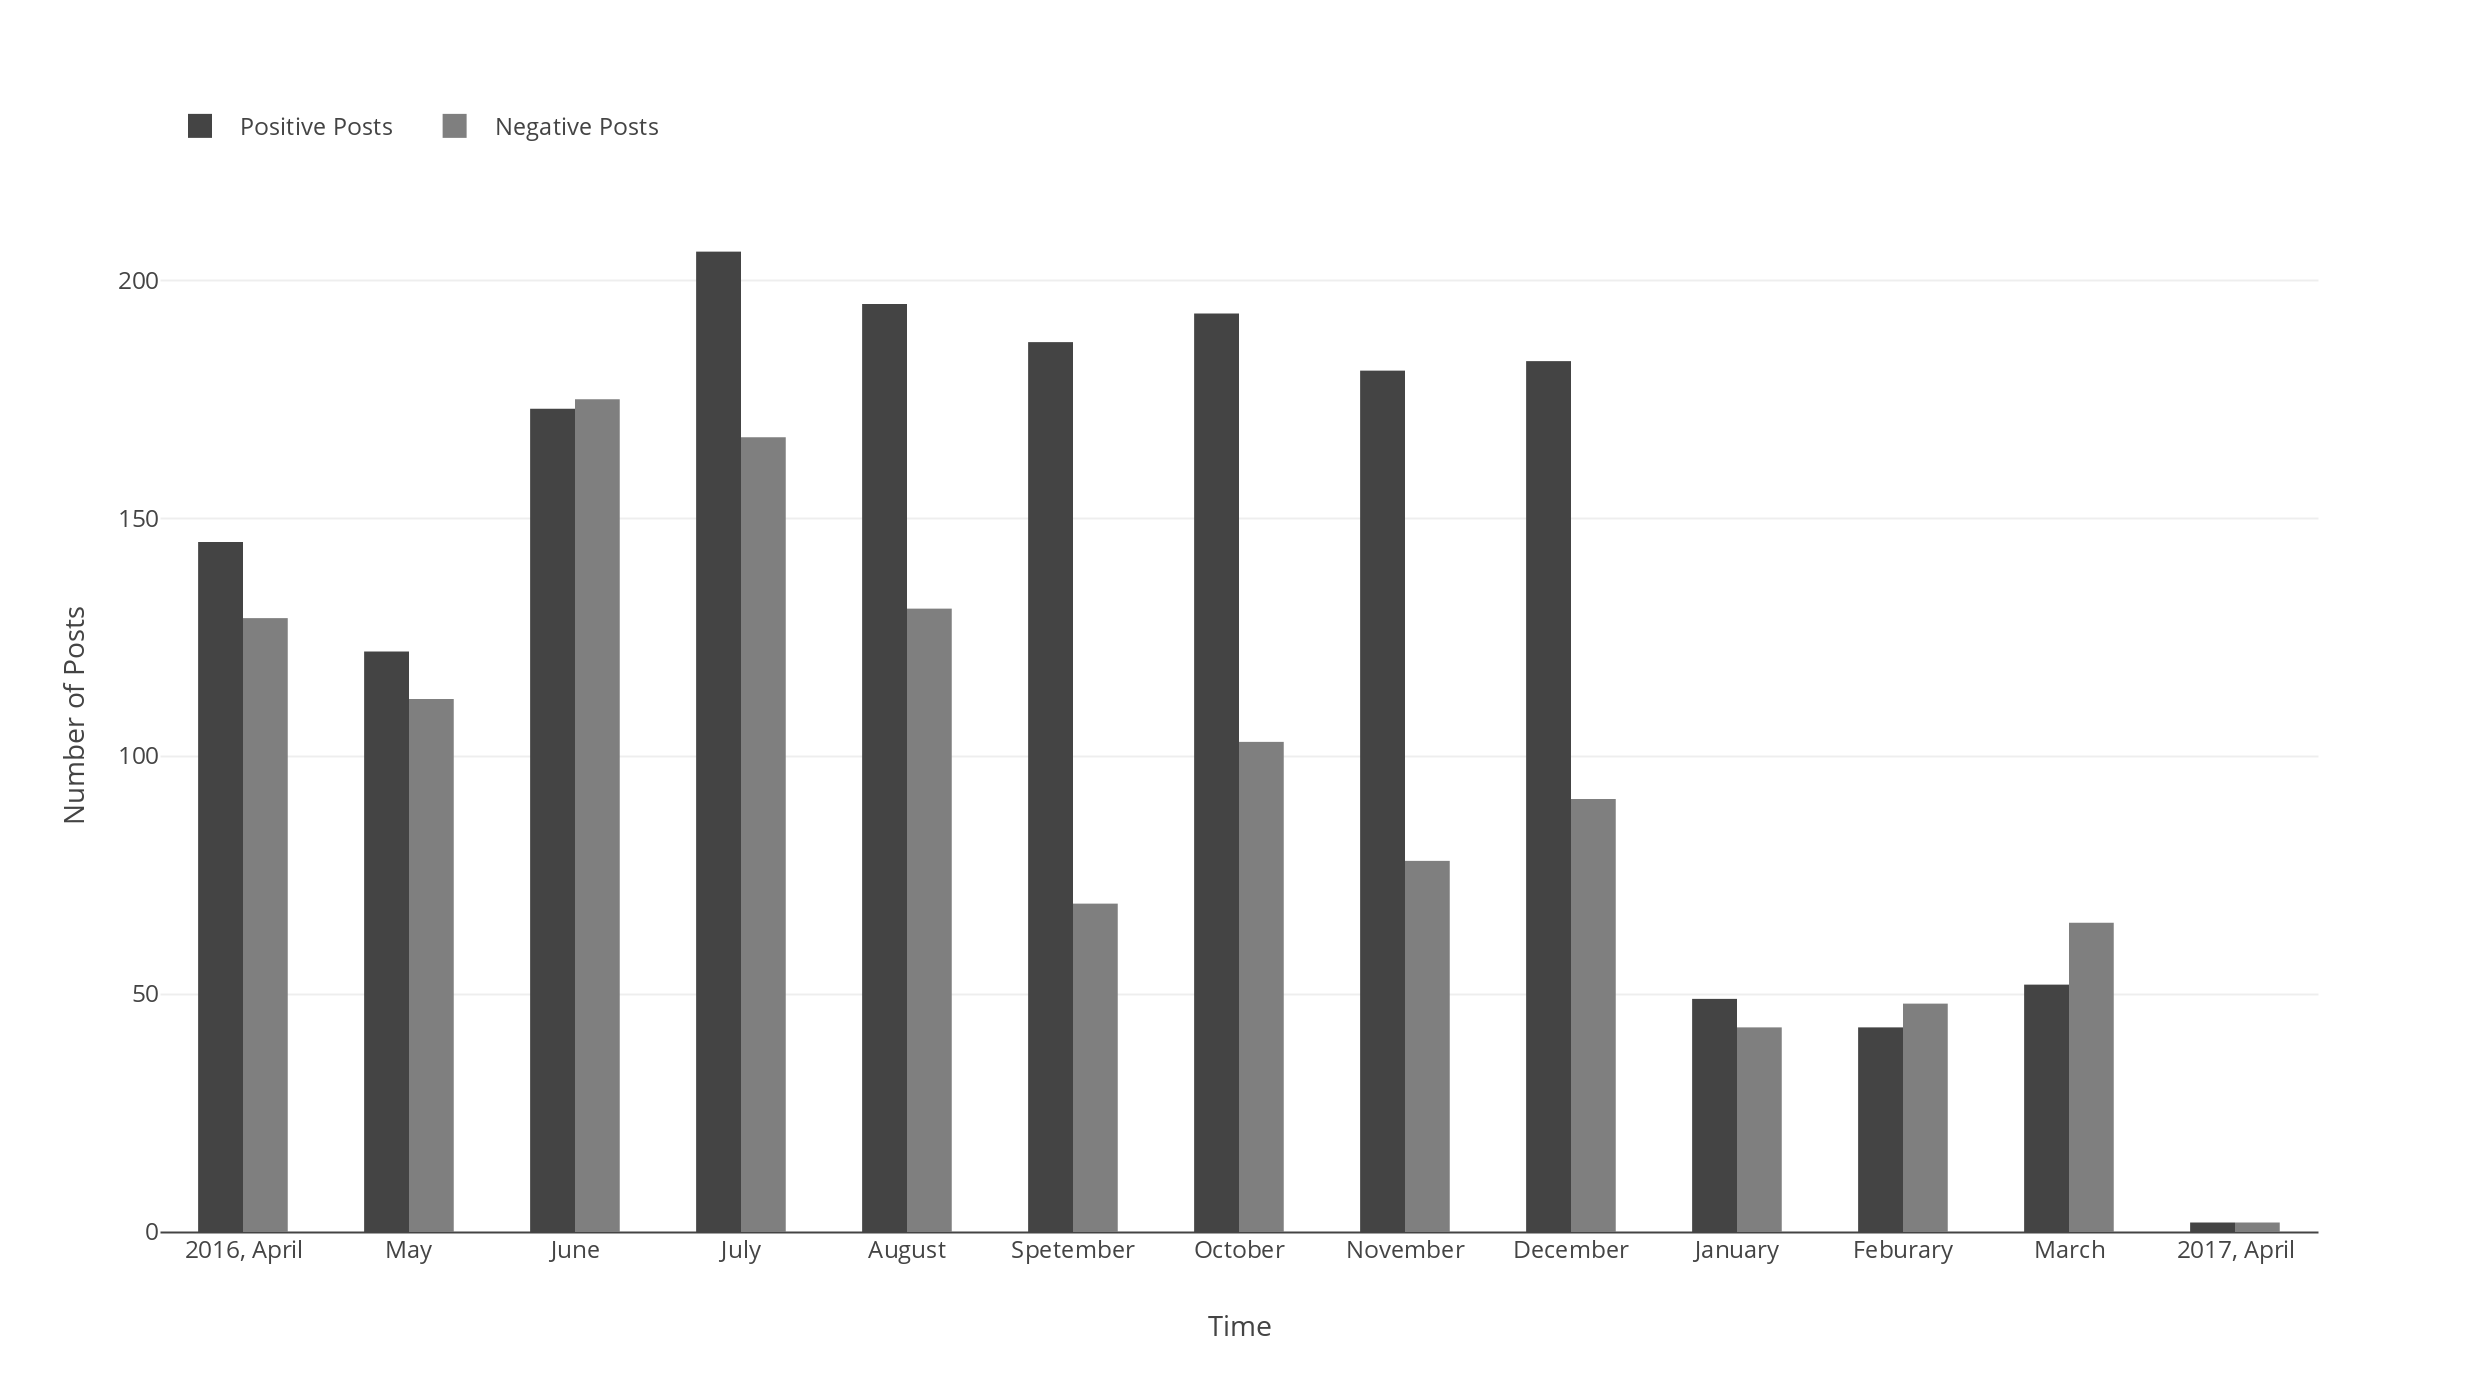
\includegraphics[width=1\textwidth]{distributionOverMonth}
\label{fig:monthlydistribution}
\caption{Distribution of Positive and Negative Posts Over the Months}
\end{figure}

For positive, and negative original posts: \% of positive  vs. negative comments

Overall, majority of the comments under positive posts have a positive tone (86.5\%), and about 13.4\% negative comments. In comparison, more than one third (37.3\%) of comments responding to negative posts have a negative tone, and 62.6\% comments have a positive tone. 

impact of time on sentiment: in general how long discussions last days? hours? Depending on that, add 

In terms of time-span, the average active time of a post is around 20 hours (std: 459 hours). The longest active time lasts more than 200 days, while a lot of posts' active time end within minutes. 

\section{Discussion}

\printbibliography

\end{document}
